\subsubsection*{A. A train problem}

\problemauthor{ Баев А.Ж.}

Ответ: $2 k (k-1) + 2 (n-k) (n-k+1)$.

Асимптотика: $O(1)$.



\subsubsection*{B. Bead garland}

\problemauthor{ Баев А.Ж.}

Количество различных гирлянд изначально равно $a_1 a_2 ... a_n$. Гирлянду длины один не выгодно объединять ни к какой другой гирлянде (вместо $a \cdot 1 < a + 1$), гирлянды большей длины наоборот выгоднее объединять между собой ($a_1 \cdot a_2 > a_1 + a_2$). Значит, выгоднее всего объединить все гирлянд, с длиной больше 1. При этом стоит обратить внимание на случай, когда имеются гирлянды только единичной длины.

Асимптотика: $O(n)$.



\subsubsection*{C. Champion}

\problemauthor{ Абдикалыков А.К.}

Вывод является буквами, ascii-код которых дан на вводе (32-й символ таблицы является пробел).

Асимптотика: $O(1)$.



\subsubsection*{D. Digits}

\problemauthor{ Абдикалыков А.К.}

Пусть $d[n][k]$ --- количество $n$-значных чисел, у которых сумма цифр равна $k$. Ясно, что если у числа отбросить последнюю цифру $z$, то получим число с суммой цифр $k - z$. Значит,
$$d[i][j] = \sum_{z=0}^{\min(9,j)} d[i-1][j-z].$$
Что легко просчитать от для всех $i$ от 1 до $n$ и $j$ от 1 до $k$. Начальные значения $d[0][0] = 1$ и $d[i][0] = 0$.

Асимптотика: $O(n k)$.



\subsubsection*{E. Elimination}

\problemauthor{ Баев А.Ж.}

Пусть $d[i][j]$ --- количество работающих участков у $i$-й жилы среди участков с $(j-m+1)$-го до $j$-го включительно, которые можно вычислить за $O(1)$ каждый:$$d[i][j] = d[i][j-1] + a[i][j] - a[i][j-m]$$
для всех $i$ от 1 до $k$ и $j$ от $m$ до $n$.
Ответом на задачу будет $\max_{m\leqslant j \leqslant n} c_j$,
где $c_j$ --- количество $d[i][j] = m$, для всех $i$ от 1 до $k$.

Асимптотика: $O(n k)$.



\subsubsection*{F. Forts}

\problemauthor{ Баев А.Ж.}

\begin{center}
\definecolor{light}{rgb}{0.85,0.85,0.85}
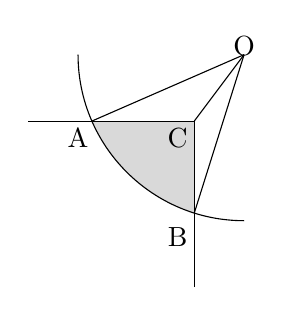
\begin{tikzpicture}[x=6, y=6]
\begin{scope}
  \clip (-10,-10) -- (-10,0) -- (0,0) -- (0, -10);
  \fill[fill=light, draw=none] (3, 4) circle (10);
\end{scope}
\draw (-7, 4) arc (180:270:10);
\draw (-10, 0) -- (0, 0);
\draw (0, -10) -- (0, 0);
\draw (3, 4) -- (0, 0);
\draw (3, 4) -- (-6.165, 0);
\draw (3, 4) -- (0, -5.539);
\node at (3, 4.5) {O};
\node at (-7, -1) {A};
\node at (-1, -7) {B};
\node at (-1, -1) {C};
\end{tikzpicture}
\end{center}

Искомая площадь равна нулю, если $a^2 + b^2 > r^2$. Иначе ее можно найти как разность площали кругового сектора $OAB$ и двух треугольников $AOC$ и $BOC$.

Асимптотика: $O(1)$.